\begin{document}

\def\lecturename{嵌入式技术}

\title{\insertlecture}

\author{邢超}

\institute
{
  西北工业大学航天学院
}

%\mode<presentation>{\subject{嵌入式系统}}

%  start a lecture  --------------------------
\lecture[EC]{嵌入式技术}{}
\subtitle{GNU/Linux 线程}
\date{2015}


%\setbeamertemplate{background}{\pgfimage[width=\paperwidth,height=\paperheight]{image/flower}}
%\setbeamercovered{transparent}
%\mode<presentation>{\beamerdefaultoverlayspecification{<+->}}

\begin{frame}
  \maketitle
\end{frame}

%\begin{frame}{课程内容}
%\begin{center}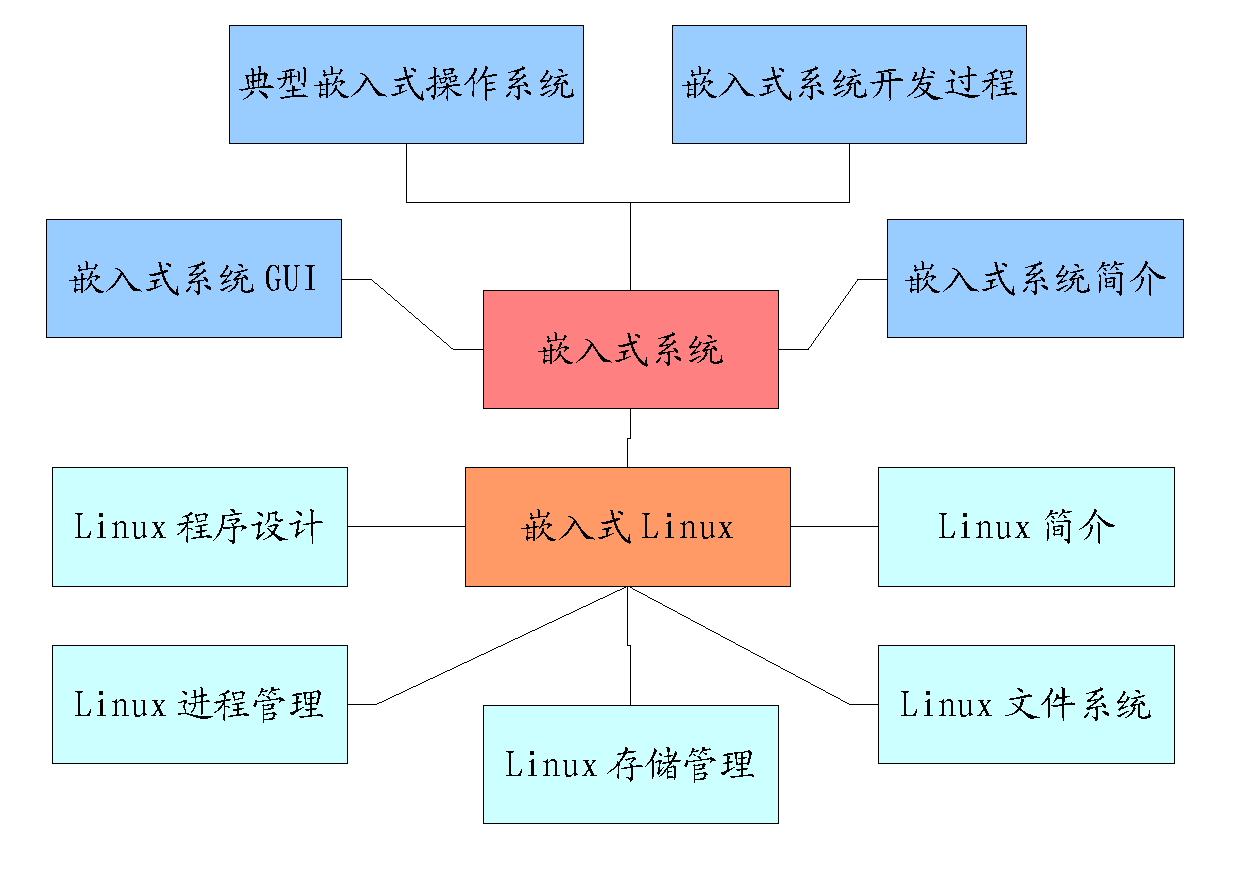
\includegraphics[height=0.8\textheight]{image/content.pdf}\end{center}
%\end{frame}


\section{线程}
\begin{frame}{线程}
\begin{itemize}
\item 线程是包含在进程中的一种实体,线程有自己的运行线索,可以完成一定的任务,可与其他线程共享进程中的共享变量及部分环境、相互之间协同来完成进程所要完成的任务。
\item 从调度的角度,线程可以分为用户线程和内核线程。
     \begin{itemize}
     \item 用户线程:用户线程的实现是通过运行时间系统代码来实现的,线程的切换实际上并不是核心调度器来实现的,而是通过进程内的代码来实现的
     \item 内核线程:内核线程切换的实现是通过内核调度器来实现的,内核线程同进程是一样的,都是核心调度器的调度实体。
     \end{itemize}
\end{itemize}
\end{frame}


\begin{frame}{线程进程比较}
     \begin{itemize}
     \item 线程和进程相比有以下优点:
          \begin{itemize}
          \item “节俭”的多任务操作方式
          \item 线程间方便的通信机制
          \item 提高应用程序响应
          \item 使多CPU系统更加有效
          \item 改善程序结构
          \end{itemize}
     \end{itemize}
\end{frame}

\begin{frame}{线程特点}
\begin{itemize}
\item 多个线程将共享同一个进程虚拟空间。线程共享的环境包括:
          \begin{itemize}
          \item 进程代码段
          \item 进程的公有数据(有利于实现线程相互之间通讯)
          \item 进程打开的文件描述符
          \item 信号的处理器
          \item 进程的当前目录
          \item 进程用户ID与进程组ID。
          \end{itemize}
\item 每个线程都具有:
          \begin{itemize}
          \item 线程ID
          \item 寄存器组的值
          \item 线程的堆栈
          \item 错误返回码
          \item 线程的信号屏蔽码
          \item 线程的优先级
          \end{itemize}
\end{itemize}
\end{frame}


\begin{frame}{Linux线程}
\begin{itemize}
\item Linux系统下的多线程遵循POSIX线程接口,称为pthread
\item 编写Linux下的多线程程序,需要使用头文件pthread.h,库文件libpthread.a
\item Linux下pthread 通过系统调用clone()来实现的
\end{itemize}
\end{frame}


\begin{frame}[containsverbatim]{threadexample1.c}
\begin{lstlisting}
#include<stdio.h>  
#include<pthread.h>
void *thread(void){
	int i;
	for(i=0;i<3;i++)
	printf("This is a pthread.\n");
}
int main(void){
	pthread_t id;
	int i,ret;
	ret=pthread_create(&id,NULL,thread,NULL);
	if(ret!=0){
		printf("Create pthread error!\n");
		exit();
	}
	for(i=0;i<3;i++) printf( \
                "This is the main process.\n");
	pthread_join(id,NULL);
	return(0);
}
\end{lstlisting}
\end{frame}


\section{互斥同步}


\begin{frame}{竟争与互斥}
\begin{center}\pgfimage[width=0.9\columnwidth]{image/share}\end{center}
\end{frame}

\begin{frame}{互斥}
     \begin{itemize}
     \item 原子操作(Atomic Operation):需要硬件的支持,架构相关; 通常用于实现资源的引用计数
     \item 自旋锁(spinlock):
           \begin{itemize}
           \item 不会引起调用者睡眠
           \item 若自旋锁已经被别的执行单元保持,调用者就一直循环在那里看是否该自旋锁已释放
           \end{itemize}
     \item 信号量(semaphore):创建时设置初始值,表示同时可以有几个任务可以访问该信号量保护的共享资源,
     \item 读写信号量(rw\_semaphore):可有任意个读者同时拥有一个读写信号量。在内核配置时,可以通过选项去控制使用哪一种实现:
           \begin{itemize}
           \item 架构无关:新的架构不需要重新实现它。性能低,获得和释放读写信号量的开销大;
           \item 架构相关:性能高,获取和释放读写信号量的开销小,但增加新的架构需要重新实现。
           \end{itemize}
     \end{itemize}
\end{frame}


\begin{frame}{多线程同步}
\begin{itemize}
\item 许多函数是不可重入的,即同时不能运行一个函数的多个拷贝
\item 在函数中声明的静态变量常常会带来一些问题,函数的返回值也会有问题
\item 共享的变量必须用关键字volatile来定义
\item 为了保护变量,必须使用信号量、互斥等方法来保证对变量的正确使用
\end{itemize}
\end{frame}


\section{思考}
\begin{frame}{思考}
\begin{itemize}
\item 进程与线程的区别
\item 线程的互斥与同步
\end{itemize}
\end{frame}

\end{document}

